% \section{SMACK Software Verification Toolchain}
% \label{sec:vmcaibackground}

% \begin{figure}[tb]
% 	\centering
% 	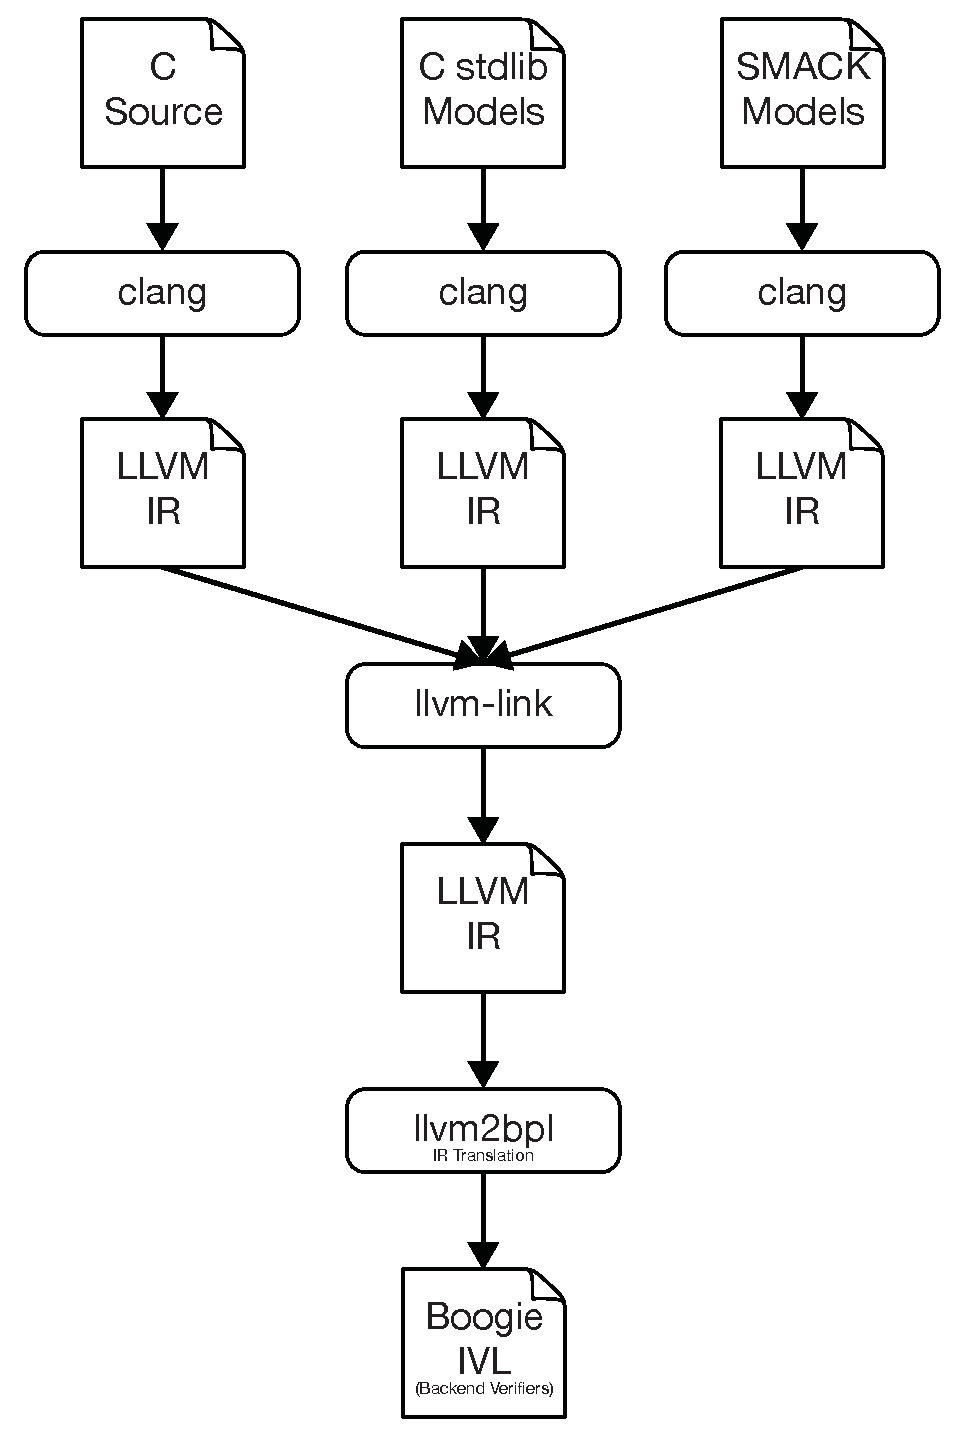
\includegraphics[width=\textwidth]{background}
% 	\caption{Toolflow of SMACK.}
% 	\label{fig:vmcaitoolflow}
% \end{figure}

% SMACK~\cite{smack-icse,smack-cav,smack-web} is an open source, modular software verification toolchain.
% %
% The core component of SMACK converts LLVM IR code into Boogie intermediate
% verification language~\cite{boogie}.
% %
% The remainder of the SMACK toolchain handles details such as compiling the
% source program into LLVM IR and invoking a Boogie verifier.
% %
% Its modular nature decouples source language details from verification by
% leveraging compiler front-ends to translate programs into the Boogie
% intermediate verification language through LLVM IR.
% %
% Before we implemented the multi-language extensions described in this chapter,
% SMACK had been predominantly used to verify LLVM IR programs produced by the
% clang C compiler.


% \cref{fig:vmcaitoolflow} shows the current toolflow of SMACK, which proceeds as
% follows:
% %
% \begin{enumerate}
% %
% \item SMACK first invokes clang, the LLVM's C compiler, to compile the input
% program, SMACK models, and C standard library models (e.g., strings, pthreads,
% math). SMACK models contain various verification primitives (e.g., for
% generating nondeterministic values) and the encoding of the memory model for
% handling of dynamically allocated memory. All of the models are written in C
% since SMACK provides a convenient mechanism for interoperating with the
% underlying Boogie code, which we describe below.
% %
% \item SMACK links together all of the generated LLVM IR files into one LLVM IR
% program.
% %
% \item The core \textsc{llvm2bpl} component of SMACK transforms an LLVM IR
% program produced by the previous step into a semantically equivalent Boogie
% program.
% %
% \item Finally, a back-end verifier, such as Corral~\cite{corral}, verifies the
% generated Boogie program using an SMT solver, such as Z3~\cite{z3}.
% %
% \end{enumerate}
% %
% In this work, we use Corral in its bounded verification mode, meaning that it
% unrolls loops and recursion up to a certain user-provided bound.


% SMACK models verifier primitives and memory models through the use of
% \lstc{\_\_SMACK\_code} function. 
% %
% This C routine takes a formatted string as a parameter, and is declared in the
% SMACK header files, but not implemented in any models. 
% %
% When \textsc{llvm2bpl} comes across a call to this function, instead of
% translating the function call, it simply inserts the parameters into the Boogie
% code snippet passed as string; this functionality is akin to C's inline
% assembly.
% %
% This allows for Boogie code or ghost variables to be injected into the
% translation, giving an easy way to encapsulate routines like \texttt{assume}
% which are not normally available in C.
% %
% It also provides an abstraction that can be used for any primitive or model.

